\documentclass{article}
% --- watermark (auto-inserted) ---
\usepackage{xcolor}
\usepackage{xfp}% \fpeval; in the kernel since 2022, harmless on older LaTeX
\usepackage{draftwatermark}
\newlength{\watermarkTextWidth}
\AddToHook{begindocument/end}{%
  \SetWatermarkText{\normalfont Generated by The Agentic Scientist}%
  \SetWatermarkFontSize{10pt}%
  \SetWatermarkLightness{0.85}%
  \settowidth{\watermarkTextWidth}{\normalfont\fontsize{10pt}{12pt}\selectfont Generated by The Agentic Scientist}%
  \edef\watermarkScale{\fpeval{0.8 * sqrt(\paperwidth**2 + \paperheight**2) / \watermarkTextWidth}}%
  \edef\watermarkAngle{\fpeval{atand(\paperheight/\paperwidth)}}%
  \SetWatermarkScale{\watermarkScale}%
  \SetWatermarkAngle{\watermarkAngle}%
}
% --- end watermark ---
 % For LaTeX2e
\usepackage{paper,times}

\usepackage{hyperref}
\usepackage{url}
\usepackage{amsmath,amssymb}
\usepackage{graphicx}
\usepackage{booktabs}
\usepackage{subcaption}

\newcommand{\Yhat}{\hat Y}
\newcommand{\E}{\mathbb{E}}
\newcommand{\Var}{\mathrm{Var}}
\newcommand{\Cov}{\mathrm{Cov}}

\title{How Much Shorter Can a Prediction-Powered Mean Interval Be? A Cross-Fitted Recalibrated Interval Is Slightly Narrower than PPI++ with Fixed Inputs}
\author{Anonymous authors}

\begin{document}
\maketitle

\begin{abstract}
Prediction-powered inference (PPI) combines a small labeled sample, a large unlabeled sample and a fixed pretrained predictor into a valid confidence interval for a population mean. We ask how much further such an interval can be shortened when labels, unlabeled data and predictor are all held fixed. Writing PPI++ as a control-variate estimator, we show that the attainable gain is governed by the gap between the squared correlation of $Y$ with $\Yhat$ and the correlation ratio of $Y$ given $\Yhat$, plus a clipping effect on the tuning weight. We evaluate a cross-fitted recalibration (isotonic or binned) added as a second control variate, with a fallback to PPI++, on a sealed evaluation of four real pools and known-truth synthetic regimes. The interval is 2.2\% narrower than PPI++ (geometric mean over five families), 6.8\% narrower than PPI with $\lambda{=}1$ and 30\% narrower than the labeled-only interval; per-family reductions range from 0.2\% to 4.0\%. Pooled coverage is 0.934 (lowest family 0.91), below the nominal 0.95 although not rejected by the evaluator's exact tests, and the observed narrowing exceeds our population-level ceiling in four of five families. The evidence supports a small, regime-dependent gain; it does not show that the gain is free of a coverage cost.
\end{abstract}

\section{Introduction}
In ecological remote sensing, galaxy morphology and census analysis, a scientist often holds three things: a small set of gold-standard labels, a large set of records without labels, and a pretrained predictor that cannot be modified. Prediction-powered inference \citep{Angelopoulos2023PredictionpoweredI} and its power-tuned form PPI++ \citep{Angelopoulos2023PPIEP} use the predictor on both samples to produce confidence intervals that remain valid for any predictor and are shorter than the labeled-only interval when the predictor is informative.

We study a deliberately narrow question. \emph{With the labeled set, the unlabeled set and the predictor all fixed, can a valid mean interval be shortened below PPI++? By how much, and under which conditions does it help or fail?} Fixing the inputs excludes active labeling \citep{Zrnic2024ActiveSI}, retraining the predictor, and adding covariates or data; the only remaining freedom is how $(Y,\Yhat)$ pairs and unlabeled predictions are turned into an interval. The labeled-only data and the predictions are all that any such interval can use.

Our route is a nested one. PPI++ is a control-variate estimator whose control variate is $\Yhat$ with a scalar weight clipped to $[0,1]$. We add a second control variate $g(\Yhat)$, a recalibration of the prediction fitted on the labeled data by cross-fitting, and let a variance-minimizing weight vector combine the two. A selection rule falls back to PPI++ unless a recalibrated interval is at least 1\% shorter than the PPI++ interval. The question then reduces to how much variance the second control variate can remove.

\paragraph{Contributions.}
\begin{itemize}
\item \textbf{Headroom analysis.} For control-variate mean intervals with fixed inputs we give the asymptotic variance in closed form (Section~\ref{sec:theory}). Relative to PPI++ the gain depends on two quantities only: the clipping of the tuning weight, and the gap $\eta^2-\rho^2$ between the correlation ratio of $Y$ on $\Yhat$ and the squared Pearson correlation. We list the conditions under which the gain is zero; a two-valued predictor removes the nonlinearity term but not necessarily the clipping term.
\item \textbf{A recalibrated PPI interval} with isotonic and binned recalibrators, cross-fitting, Student-$t$ critical values and a 1\%-margin fallback to PPI++ (Section~\ref{sec:method}).
\item \textbf{A sealed evaluation} on four real pools and four known-truth synthetic regimes, scored against classical, PPI ($\lambda{=}1$) and PPI++ intervals, with the width gain, the coverage evidence and the population-level ceiling reported side by side (Section~\ref{sec:results}).
\item \textbf{A calibrated conclusion.} The recalibrated interval is narrower than PPI++ by 2.2\% on average, but the average exceeds the population-level ceiling and coverage point estimates sit below 0.95. We state precisely what the evidence does and does not support (Section~\ref{sec:discussion}).
\end{itemize}

\begin{figure}[t]
\centering
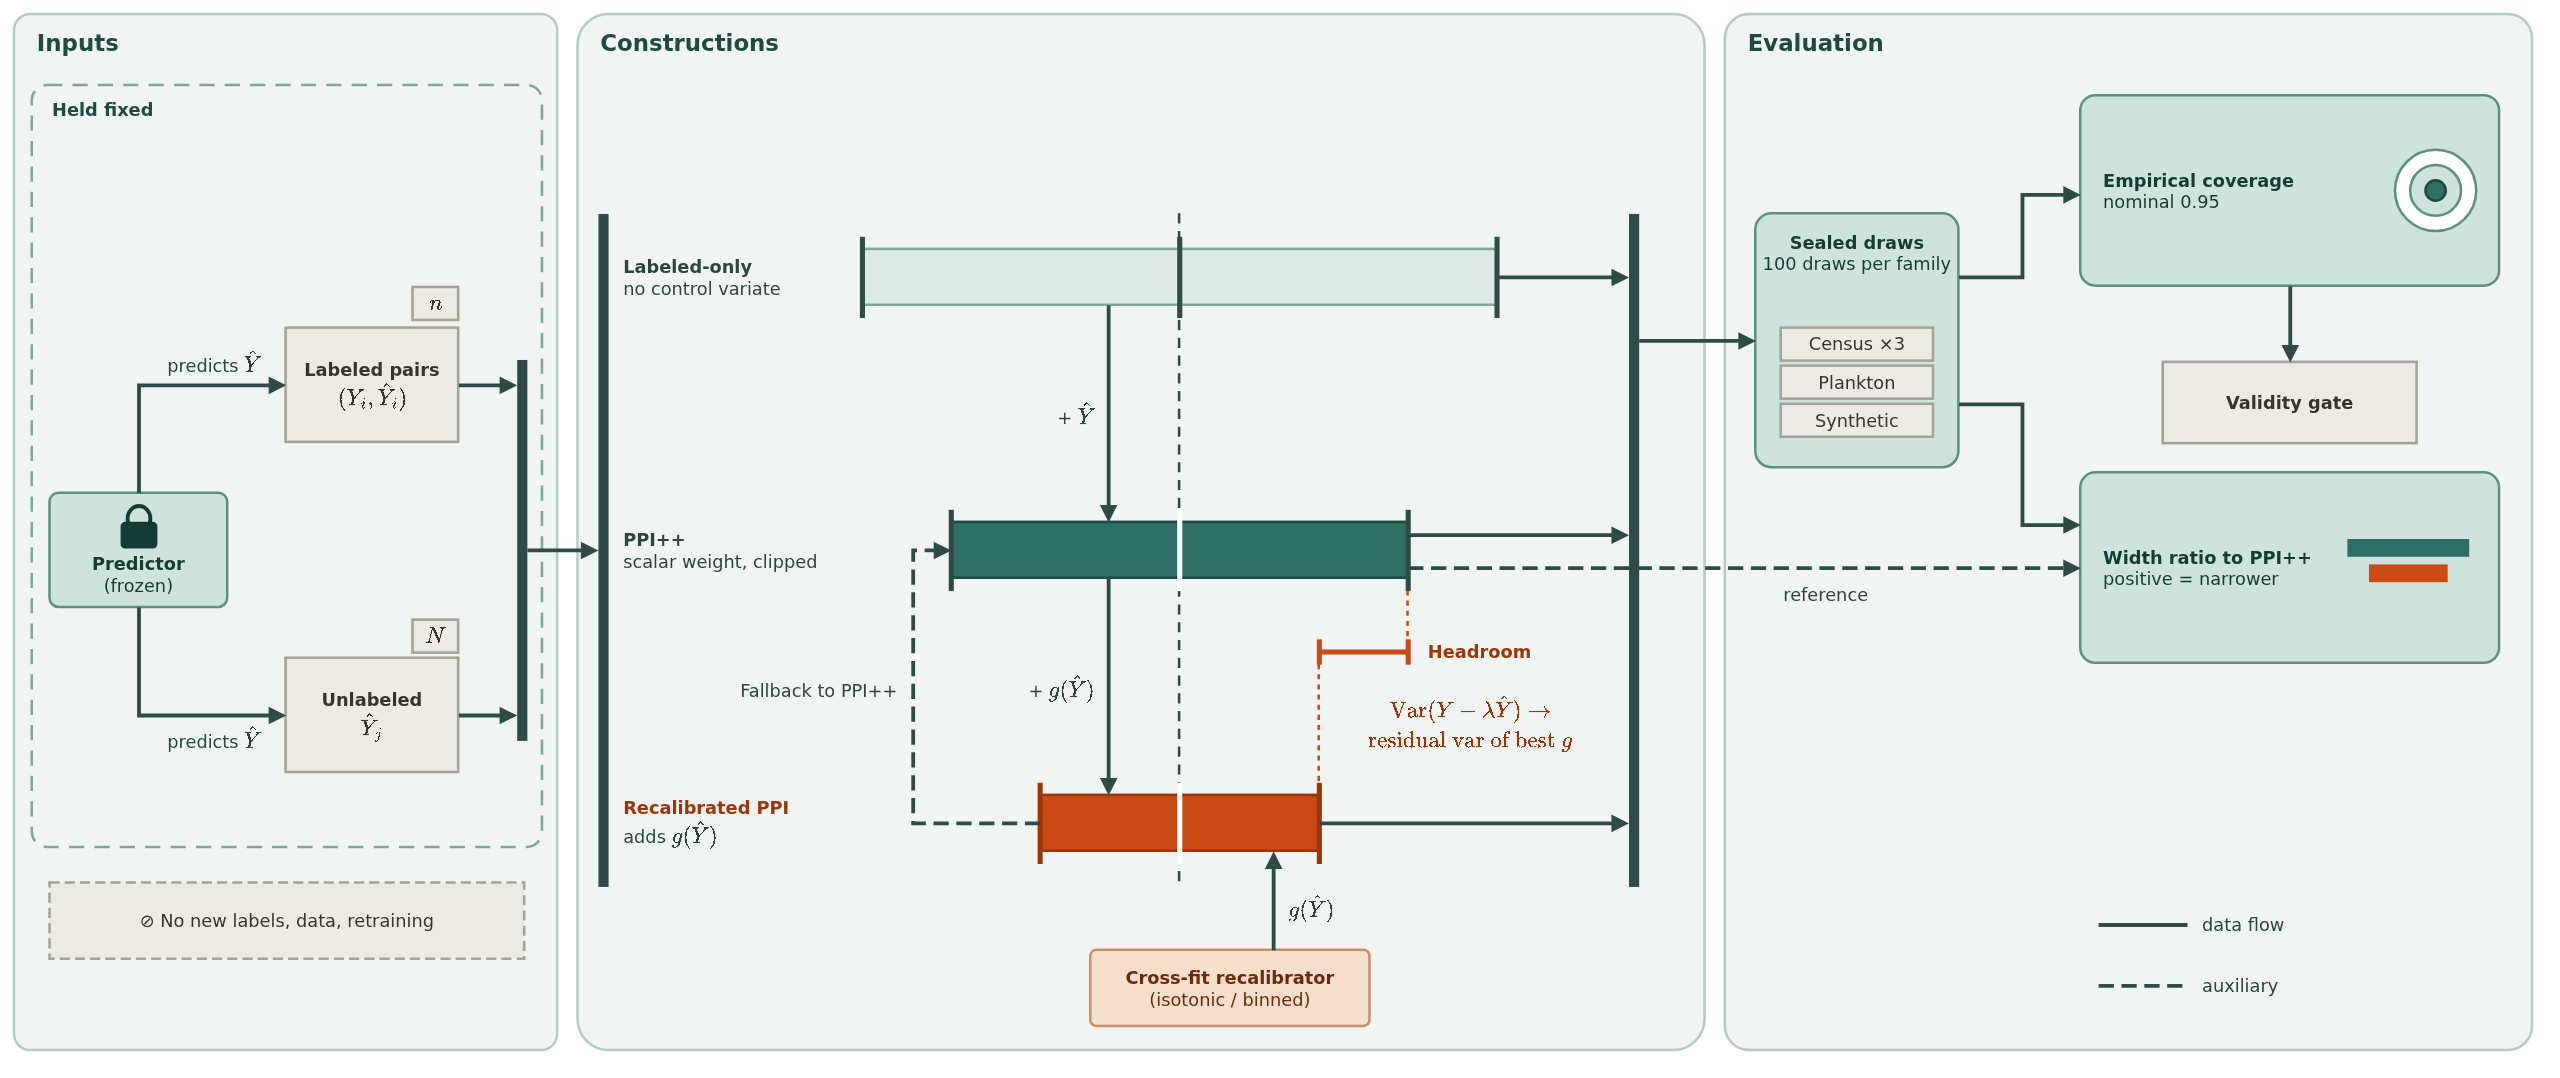
\includegraphics[width=\textwidth]{figures/overview_setting_and_method.png}
\caption{Setting and compared constructions. With labels, unlabeled records and the predictor fixed, three intervals are built from the same data: the labeled-only interval, PPI++ (scalar weight on $\Yhat$), and recalibrated PPI (cross-fitted $g(\Yhat)$ as an additional control variate, with a fallback to PPI++). Each is scored by empirical coverage and by the width ratio to PPI++; the achievable narrowing is bounded by the drop from $\Var(Y-\lambda\Yhat)$ to the residual variance of the best $g$.}
\label{fig:overview}
\end{figure}

\section{Related Work}
\paragraph{Prediction-powered inference.} PPI \citep{Angelopoulos2023PredictionpoweredI} corrects a prediction-based estimate with a rectifier measured on labeled data; PPI++ \citep{Angelopoulos2023PPIEP} tunes a scalar weight to minimize the interval width and is our primary comparator. Cross-prediction-powered inference \citep{Zrnic2023CrosspredictionpoweredI} handles predictors trained on the same labeled data by cross-fitting, a device we reuse for the recalibration map. Stratified PPI \citep{Fisch2024StratifiedPI} corrects within strata of the predictor output; we include an implementation as a reference estimator but report no results for it. Further variants cover imputed covariates and nonuniform sampling \citep{Kluger2025PredictionPoweredIW}, e-values \citep{Csillag2025PredictionPoweredE}, Bayesian and Bayes-assisted constructions \citep{Hofer2024BayesianPI,Kilian2025AnytimevalidBI,Cortinovis2025FABPPIFA}, adaptive shrinkage \citep{Li2025PredictionPoweredAS}, local and sparse regression settings \citep{Gu2024LocalPI,Song2025SparseEA}, federated data \citep{Luo2024FederatedPI}, causal estimands \citep{Cadei2025PredictionPoweredCI}, risk control \citep{Einbinder2024SemiSupervisedRC}, clinical trials \citep{Poulet2025PredictionpoweredIF}, wireless systems \citep{Sifaou2024SemiSupervisedLV} and satellite-based poverty analysis \citep{Pettersson2025DebiasingML}. These works change the estimand, the sampling design or the inferential framework; we instead ask how much a plain mean interval can still be shortened with the inputs fixed.

\paragraph{Semi-supervised and debiased estimation.} The control-variate form of PPI has antecedents in the classical use of control variables to reduce estimator variance \citep{Lavenberg1981Perspective}, in augmented inverse-probability-weighted estimation with missing outcomes \citep{Robins1994Estimation,Bang2005Doubly}, in semi-supervised mean estimation \citep{Zhang2016SemisupervisedIG} and in semiparametrically efficient semi-supervised learning \citep{Xu2025AUF}, where efficiency is characterized through the conditional mean of the outcome. Our headroom formula (Section~\ref{sec:theory}) is a finite-$n/N$ restatement of this efficiency logic for the case where the only available function of the data is $\Yhat$; we do not claim it as a new efficiency result, and we did not verify it against these sources beyond the qualitative correspondence. Debiased machine learning with cross-fitted nuisance estimates \citep{Chernozhukov2017DoubledebiasedML} supplies the template for using an estimated conditional mean inside a valid interval. Our setting differs in that the covariates are not available and the only usable function of the data is $\Yhat$.

\paragraph{Calibration.} Isotonic and binned maps from scores to outcome probabilities are standard calibration tools \citep{Zadrozny2002TransformingCS,Niculescu-Mizil2005PredictingGP}. Isotonic regression also extends beyond probabilities to monotone conditional-distribution estimation for general real-valued outcomes \citep{Henzi2021Isotonic}. Here the maps estimate $\E[Y\mid \Yhat]$ for use as a control variate, not to produce probabilities.

\section{Method}\label{sec:method}
\subsection{Problem setup}
Let $(Y_i,\Yhat_i)$, $i=1,\dots,n$ be labeled pairs and $\Yhat_j$, $j=1,\dots,N$ unlabeled predictions, all i.i.d.\ from one population, with a fixed predictor producing $\Yhat$. The target is $\theta=\E[Y]$, the mean estimand, and the interval must have coverage at least $1-\alpha$ with $\alpha=0.05$ under repeated sampling. We write $r=n/N$. The objective is the interval width at maintained coverage. No additional labels, data or predictor changes are allowed, and no covariates enter beyond $\Yhat$.

\subsection{Control-variate view and headroom}\label{sec:theory}
For a feature vector $f(\Yhat)\in\mathbb{R}^p$ and weights $\lambda\in\mathbb{R}^p$ define
\begin{equation}
\hat\theta_\lambda=\frac1N\sum_{j=1}^N\lambda^\top f(\Yhat_j)+\frac1n\sum_{i=1}^n\bigl(Y_i-\lambda^\top f(\Yhat_i)\bigr),
\end{equation}
which is unbiased for fixed $\lambda$ and $f$. Its asymptotic variance satisfies $n\,V(\lambda)=\Var(Y)-2\lambda^\top c+(1+r)\lambda^\top\Sigma\lambda$ with $c=\Cov(f,Y)$ and $\Sigma=\Var(f)$, minimized at $\lambda^\star=\Sigma^{-1}c/(1+r)$:
\begin{equation}
n\,V^\star=\Var(Y)\Bigl(1-\frac{R_f^2}{1+r}\Bigr),\qquad R_f^2=\frac{c^\top\Sigma^{-1}c}{\Var(Y)}.
\label{eq:vstar}
\end{equation}
Here $f=0$ gives the labeled-only interval, $f=\Yhat$ with $\lambda=1$ gives PPI, and $f=\Yhat$ with the estimated weight clipped to $[0,1]$ gives PPI++ (the clip is applied in the reference implementation we compare against; Supplement~\ref{sec:si-source}). With an unclipped weight on $\Yhat$ the explained share is $R_f^2=\rho^2$, the squared Pearson correlation. If the feature set contains $m(\Yhat)=\E[Y\mid\Yhat]$ then $R_f^2=\eta^2:=\Var(m(\Yhat))/\Var(Y)$, the correlation ratio. Hence the oracle standard-error ratio between a recalibrated and an unclipped-linear interval is
\begin{equation}
\sqrt{\frac{1-\eta^2/(1+r)}{1-\rho^2/(1+r)}},\qquad\text{which tends to }\sqrt{\frac{1-\eta^2}{1-\rho^2}}\text{ as }r\to0.
\label{eq:ceiling}
\end{equation}
Two things can therefore shorten a PPI++ interval with fixed inputs: allowing the weight to leave $[0,1]$ when the unclipped optimum $\lambda^\star>1$, and capturing nonlinearity of $\E[Y\mid\Yhat]$, measured by $\eta^2-\rho^2\ge0$. The gain is \emph{zero} when (i) $\E[Y\mid\Yhat]$ is affine in $\Yhat$, which includes every predictor taking only two values, since two points are always collinear (this removes the nonlinearity term only; the total gain is then zero provided the unclipped optimal weight also lies in $[0,1]$); (ii) $\Yhat$ is uninformative ($\rho=\eta=0$); or (iii) $n$ is small enough that estimating $g$ costs more variance than it removes, a loss of order $p/n$ in relative variance. These are asymptotic statements for fixed $g$; with a cross-fitted $\hat g$ they require that $\hat g$ converge to $m$ at an adequate rate, which we assume and do not prove here (derivation in Supplement~\ref{sec:si-deriv}).

\subsection{Compared estimators}
Table~\ref{tab:estimators} lists the interval constructions. All use $\alpha=0.05$ and an estimated standard error from the labeled residual and the unlabeled control-variate term.

\begin{table}[t]
\centering
\caption{Interval constructions compared. ``Weight'' is the control-variate weight on the listed features.}
\label{tab:estimators}
\small
\begin{tabular}{p{2.6cm}p{2.9cm}p{3.1cm}p{3.6cm}}
\toprule
Interval & Features & Weight & Critical value / notes \\
\midrule
Labeled-only & none & --- & normal; uses labels only \\
PPI & $\Yhat$ & $\lambda{=}1$ & normal \\
PPI++ & $\Yhat$ & scalar, estimated, clipped to $[0,1]$ & normal; primary comparator, also the fallback \\
Stratified PPI & quantile strata of $\Yhat$ & $\lambda{=}1$ per stratum & normal; implemented, no reported results \\
Recalibrated PPI (studied) & $\Yhat$ and cross-fitted $g(\Yhat)$ & vector, estimated, unclipped & Student-$t$, $n{-}1{-}p$ d.f.; adopted only if $\ge1\%$ shorter than PPI++ \\
\bottomrule
\end{tabular}
\end{table}

\subsection{Cross-fitted recalibrated PPI}
Let $K=5$. Labeled indices are split at random into $K$ folds. For each fold, a recalibrator $g^{(k)}$ is fitted on the other folds. Out-of-fold values $g^{(k)}(\Yhat_i)$ are used on the held-out labeled points, and the average $K^{-1}\sum_k g^{(k)}(\Yhat_j)$ is used on the unlabeled points. Two recalibrators are used: an isotonic fit whose direction follows the sign of the sample correlation, and a quantile-binned conditional mean with $\min(10,\max(2,\lfloor 0.8n/25\rfloor))$ bins. The two features $(\Yhat,g)$ are standardized with their pooled mean and standard deviation, and the weight solves $\lambda=(\hat\Sigma_\ell+r\hat\Sigma_u+\epsilon I)^{-1}\hat c$ with a small ridge $\epsilon$. The interval is the control-variate estimate plus or minus a Student-$t$ quantile with $n-1-p$ degrees of freedom ($p=2$) times $\sqrt{s_u^2/N+s_\ell^2/n}$, where $s_\ell^2$ is the residual variance on labeled points and $s_u^2$ the variance of the weighted control variate on unlabeled points.

\paragraph{Selection with fallback.} The PPI++ interval is computed first. A recalibrated candidate is adopted only if its half-width is below 0.99 times the PPI++ half-width. The isotonic candidate is tried first and the binned candidate second; once the isotonic candidate has been adopted, the binned candidate replaces it if it is merely narrower, with no additional margin. If neither candidate passes the test against PPI++, PPI++ is returned. If $n<20$ or $\Yhat$ is constant, no candidate is formed. The 1\% margin is a heuristic guard against selection noise, not a validity guarantee; the interval chosen by comparing estimated widths is data-dependent, and the standard-error estimate does not account for the estimation of $g$ or of $\lambda$ beyond the degrees-of-freedom correction.

\subsection{Evaluation protocol}
\paragraph{Pools and draws.} The sealed evaluation uses four real pools, each with $n=500$ labeled and $N=20000$ unlabeled records: California census income, census private-insurance indicator, a census education-related quantity (all with model predictions; census tabular benchmarks of the kind assembled by \citealt{Ding2021RetiringAN}), and a plankton-imaging pool whose prediction takes only two values. A fifth family is synthetic with four regimes (linear calibrated, nonlinear miscalibrated with a cubic predictor, uninformative, heteroscedastic), $n\in\{200,500\}$ and $N\in\{2000,20000\}$. Each family has 100 independent draws; real-pool draws are taken with replacement from the pool, so the truth is the pool mean, and synthetic truths are analytic. Controls with a constant predictor, a permuted predictor and a shifted outcome are run separately.

\paragraph{Score and validity gate.} For each family $f$ the evaluator forms $s_f=-\log(\sum_e W_e/\sum_e P_e)$ from candidate widths $W_e$ and PPI++ widths $P_e$ over its episodes (positive means narrower), and averages $s_f$ over the five families. The same construction against PPI ($\lambda{=}1$) and the labeled-only interval gives the other two comparators; baselines come from ppi-python 0.2.3. Validity requires non-rejection of nominal coverage by exact one-sided binomial tests (pooled level 0.01, per-family level $0.01/5$, failed episodes counted as misses with worst-case width) and all controls passing. A paired episode-level bootstrap of the aggregate score (2000 replicates) must have a positive 2.5th percentile for the narrowing to be declared. Non-rejection is a weaker statement than coverage equal to nominal.

\paragraph{Design-space contrast.} Before the sealed evaluation, three model variants were scored once each on separate search pools (galaxy morphology, Amazon deforestation, gene expression, protein disorder, plus synthetic regimes; 60 draws per family): the recalibrated interval above, a label-free spline-basis control variate with leave-one-out PRESS model selection, and a repeated-cross-fitted calibrator stack combined by non-negative least squares. These are single evaluations on search pools and are reported as a contrast in Section~\ref{sec:search}, not as controlled ablations; the search pools are disjoint from the sealed pools.

\section{Results}\label{sec:results}
\subsection{Validity: coverage evidence}\label{sec:validity}
The sealed evaluation completed with all controls passed, zero failed episodes, and the validity gate and the bootstrap criterion satisfied (final outcome \emph{qualified}). Pooled empirical coverage over the 500 evaluated draws is 0.934 (467 covered) and the lowest family coverage is 0.91 (91 of 100). % @evidence[[paper_data.json#final_evaluation.metrics.coverage_pooled]] @evidence[[paper_data.json#final_evaluation.metrics.coverage_min_family]] @evidence[[paper_data.json#final_evaluation.metrics.controls_passed]] @evidence[[paper_data.json#final_evaluation.metrics.n_failed_episodes]]
Both point estimates lie below the nominal 0.95. Under exact binomial calculations with $p=0.95$, the lower-tail probabilities of the observed counts are 0.066 (pooled) and 0.063 (lowest family), % @evidence[[analysis/headroom_derived.json#coverage]]
which is why the gate did not reject, but also not strong support for exact nominal coverage; the Monte Carlo standard errors are 0.011 and 0.029. % @evidence[[analysis/headroom_derived.json#coverage]]
Coverage of the PPI++ and labeled-only baselines was not recorded in the available artifacts, and per-family coverage other than the minimum is unavailable. We therefore cannot say whether the shortfall is a property of recalibration, of finite-sample Wald intervals at these sample sizes, or of the data-dependent selection step.

\subsection{Width: sealed final evaluation}
Figure~\ref{fig:final} and Table~\ref{tab:final} give the width results. Against PPI++ the mean log width ratio is 0.022, i.e.\ the geometric-mean interval is 2.2\% narrower (derived as $1-e^{-0.022}$). % @evidence[[paper_data.json#final_evaluation.metrics.combined_score]]
Against PPI with $\lambda{=}1$ the mean log ratio is 0.070 (6.8\% narrower) and against the labeled-only interval 0.358 (30\% narrower). % @evidence[[paper_data.json#final_evaluation.metrics.log_ratio_vs_ppi_lambda1_mean]] @evidence[[paper_data.json#final_evaluation.metrics.log_ratio_vs_classical_mean]]
Most of the gain over labeled-only inference is therefore already captured by PPI machinery; recalibration adds a small increment on top. Per family, the narrowing against PPI++ is 0.0287 for census income, 0.0018 for census insurance, 0.0023 for census education, 0.0359 for plankton and 0.0413 for the synthetic mixture, corresponding to derived width reductions of 2.8\%, 0.2\%, 0.2\%, 3.5\% and 4.0\%. % @evidence[[paper_data.json#final_evaluation.metrics]] @evidence[[analysis/headroom_derived.json#derived_width_reduction_vs_ppi_pp]]
No family is wider than PPI++ on this measure, but the gain is near zero for two of five families.

\begin{figure}[t]
\centering
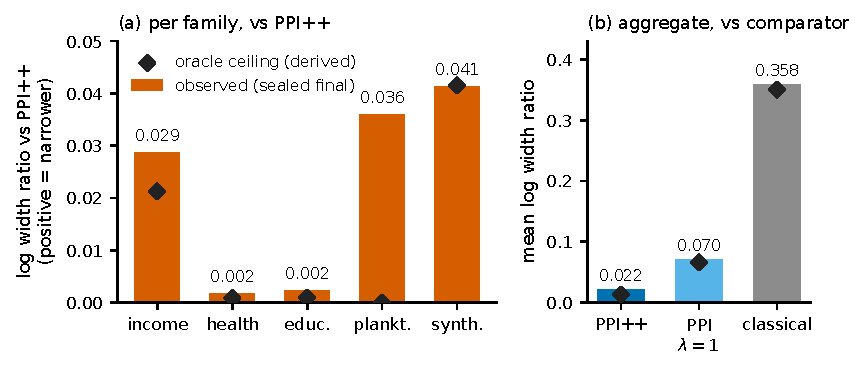
\includegraphics[width=\textwidth]{figures/final_width_ratio.pdf}
\caption{Sealed final width results. (a) Observed log width ratio against PPI++ by family (bars; positive means narrower than PPI++) and the population-level oracle ceiling of Eq.~\eqref{eq:ceiling} (diamonds, derived from the pools). (b) Aggregate mean log ratio against the three comparators, with the aggregate ceiling. Single sealed evaluation; no confidence intervals are available for the ratios.}
\label{fig:final}
\end{figure}

\begin{table}[t]
\centering
\caption{Sealed final results by family: observed log width ratio against PPI++, derived percent reduction, oracle ceiling of Eq.~\eqref{eq:ceiling} on the pool (derived), the part of the ceiling reachable by an unclipped linear weight, and the excess of observed over ceiling. Aggregate row: mean over families.}
\label{tab:final}
\small
\begin{tabular}{lrrrrr}
\toprule
Family & Observed & Reduction & Ceiling & Unclipped-linear part & Observed $-$ ceiling \\
\midrule
census income & 0.0287 & 2.8\% & 0.0213 & 0.0179 & 0.0074 \\
census insurance & 0.0018 & 0.2\% & 0.0008 & 0.0000 & 0.0009 \\
census education & 0.0023 & 0.2\% & 0.0009 & 0.0000 & 0.0014 \\
plankton & 0.0359 & 3.5\% & 0.0000 & 0.0000 & 0.0359 \\
synthetic & 0.0413 & 4.0\% & 0.0416 & 0.0000 & $-$0.0003 \\
\midrule
aggregate & 0.0220 & 2.2\% & 0.0129 & 0.0036 & 0.0091 \\
\bottomrule
\end{tabular}
% @evidence[[paper_data.json#final_evaluation.metrics]] @evidence[[analysis/headroom_derived.json#oracle_vs_ppi_pp]] @evidence[[analysis/headroom_derived.json#oracle_linear_vs_ppi_pp]]
\end{table}

\subsection{How does the observed gain compare with the population-level ceiling?}\label{sec:headroomcheck}
We evaluated Eq.~\eqref{eq:ceiling} on each pool, using $\rho^2$ and an isotonic estimate of $\eta^2$ on the full pool, $n=500$, $N=20000$, and the evaluator's PPI++ weight clip (for synthetic regimes, large-sample moments of the generator and the evaluator's episode plan). The population ceiling is not a bound on a single finite draw, and it excludes the estimation cost of $g$.

\emph{Where the ceiling is positive, it is small.} The ceiling against PPI++ is 0.0213 for census income, 0.0008 and 0.0009 for the two other census pools, and 0.0416 for the synthetic mixture; the aggregate is 0.0129. % @evidence[[analysis/headroom_derived.json#oracle_vs_ppi_pp]] @evidence[[analysis/headroom_derived.json#oracle_aggregate_vs_ppi_pp]]
For census income, the unclipped optimal weight computed from the pool is 1.34 (the clipped weight equals 1), and 0.0179 of the 0.0213 ceiling is reachable by an unclipped linear weight on $\Yhat$ alone; the pool's $\eta^2$ and $\rho^2$ differ by only 0.0044. % @evidence[[analysis/headroom_derived.json#oracle_linear_vs_ppi_pp]] @evidence[[analysis/headroom_derived.json#real.census_income]]
So for this pool the population-level ceiling is mostly reachable by an unclipped linear weight rather than by nonlinear recalibration; this describes the ceiling, not the source of the evaluated interval's observed gain, which was not isolated. For the synthetic family, the entire ceiling comes from the nonlinear-miscalibrated regime ($\eta^2=0.71$ against $\rho^2=0.48$), and the observed 0.0413 matches the ceiling 0.0416 within 0.0003. % @evidence[[analysis/headroom_derived.json#synthetic_regimes]]

\emph{Where the observed gain exceeds the ceiling.} In four of five families the observed narrowing is larger than the ceiling (Table~\ref{tab:final}). The plankton pool is the clearest case: the predictor takes only two values, so $\E[Y\mid\Yhat]$ is affine in $\Yhat$, the unclipped optimal weight (0.841) lies inside $[0,1]$, the ceiling is zero, yet the observed narrowing is 0.0359 (3.5\%). % @evidence[[analysis/headroom_derived.json#real.plankton]] @evidence[[paper_data.json#final_evaluation.metrics.log_ratio_vs_ppi_family_plankton]]
The aggregate observed value 0.0220 exceeds the aggregate ceiling 0.0129 by 0.0091. The same holds against PPI with $\lambda{=}1$ (0.0701 observed, 0.0661 ceiling) and against the labeled-only interval (0.3581 observed, 0.3498 ceiling). % @evidence[[analysis/headroom_derived.json#oracle_aggregate_vs_ppi_lam1]] @evidence[[analysis/headroom_derived.json#oracle_aggregate_vs_classical]]
Asymptotic variance reduction from recalibration cannot account for this part. We did not run a diagnostic that isolates its source. Candidate explanations, none tested here, are (a) finite-sample optimism of an interval whose weight and residual variance are estimated on the same labeled data, (b) selection of the narrowest of three estimated widths (PPI++ and the isotonic and binned candidates, with a 1\% margin required only relative to PPI++), which favors downward noise in the estimated standard error, and (c) differences in finite-sample variance estimation between the evaluated implementation and the reference baseline. Explanations (a) and (b) would also lower coverage and are consistent with the coverage shortfall of Section~\ref{sec:validity}, but the available artifacts do not allow us to establish that link. For the two census pools with near-zero ceilings, the excess is 0.0009 and 0.0014; with no per-episode widths in the artifacts, we cannot tell whether it is distinguishable from pairing noise.

\emph{Regime-level headroom is much larger than the family-level average.} Within the nonlinear-miscalibrated synthetic regime alone, the same formula gives an oracle narrowing over an unclipped linear weight of 0.286 in log width for $(n,N)=(200,20000)$ and 0.178 for $(500,2000)$ (Table~\ref{tab:rsens}), i.e.\ roughly 25\% to 16\% shorter intervals; the gain falls as $r=n/N$ grows because the unlabeled sample then carries less of the variance. The family-level ceiling of 0.0416 is much smaller because three of the four regimes have no headroom and the evaluator's ratio of summed widths weights the nonlinear regime by its (smallest) interval width. For census income the same calculation gives at most 0.0034 over an unclipped linear weight, whatever $r$. % @evidence[[analysis/headroom_derived.json#oracle_recal_over_linear_by_cell]]

\begin{table}[t]
\centering
\caption{Oracle recalibration gain over an unclipped linear weight on $\hat Y$ (log width ratio, Eq.~\eqref{eq:ceiling}) by sample-size cell, for the one synthetic regime with nonlinear calibration and for the census-income pool (derived).}
\label{tab:rsens}
\small
\begin{tabular}{lrrrr}
\toprule
 & $(200,20000)$ & $(500,20000)$ & $(200,2000)$ & $(500,2000)$ \\
$r=n/N$ & 0.010 & 0.025 & 0.100 & 0.250 \\
\midrule
synthetic, nonlinear regime & 0.2855 & 0.2750 & 0.2323 & 0.1776 \\
census income & 0.0034 & 0.0034 & 0.0030 & 0.0025 \\
\bottomrule
\end{tabular}
% @evidence[[analysis/headroom_derived.json#oracle_recal_over_linear_by_cell]]
\end{table}

\subsection{Stability across evaluator partitions}
The evaluator also reports the aggregate score separately for five partitions of the episodes, defined by the candidate reset seed: 0.0247, 0.0220, 0.0203, 0.0213 and 0.0235, all positive. % @evidence[[paper_data.json#final_evaluation.evaluation_evidence.episodes]]
These values are a spread, not a confidence interval: the data draws do not depend on the reset seed, and because of the evaluator's episode ordering each partition contains 76 episodes of one family and six of each other family, so partitions differ in composition (Supplement~\ref{sec:si-partition}). % @evidence[[analysis/headroom_derived.json#partition_composition_main_episodes]]

\subsection{Design-space contrast on the search pools}\label{sec:search}
Figure~\ref{fig:search} compares the three model variants, each evaluated once on the search pools. Their aggregate scores against PPI++ are 0.0271 (recalibrated isotonic/binned), 0.0223 (stacked calibration) and 0.0046 (label-free basis with PRESS); all three were scored and passed the evaluator's validity gate. % @evidence[[paper_data.json#grounding_sources.result.top_program_01]] @evidence[[paper_data.json#grounding_sources.result.top_program_02]] @evidence[[paper_data.json#grounding_sources.result.top_program_03]]
The recalibrated variant is largest on the synthetic family (0.0757) and gene expression (0.0290), and smallest on galaxy morphology (0.0035). % @evidence[[source_evidence/search_metrics/recalibrated_metrics.json]]
The stacked variant tracks it on the synthetic family (0.0707) and gene expression (0.0278) but is smaller on deforestation and protein disorder; the smooth label-free basis is close to PPI++ on the synthetic family (0.0034), where the nonlinearity is the exponential regime of the search generator. % @evidence[[source_evidence/search_metrics/stacked_metrics.json]] @evidence[[source_evidence/search_metrics/label_free_basis_metrics.json]]
Search-pool pooled coverage was 0.943 for the recalibrated and the stacked variants and 0.950 for the basis variant, with minimum family coverage 0.933, 0.917 and 0.933 respectively. % @evidence[[source_evidence/search_metrics/recalibrated_metrics.json]] @evidence[[source_evidence/search_metrics/stacked_metrics.json]] @evidence[[source_evidence/search_metrics/label_free_basis_metrics.json]]
These are single evaluations without uncertainty estimates, and the variants differ in several components at once (recalibrator class, variance estimator, selection rule), so the contrast cannot attribute the difference to any one component. The stacked variant scored lower than the simpler recalibrated variant on the aggregate (0.0223 against 0.0271). We computed no headroom ceilings for the search pools, so we offer no explanation of this difference.

\begin{figure}[t]
\centering
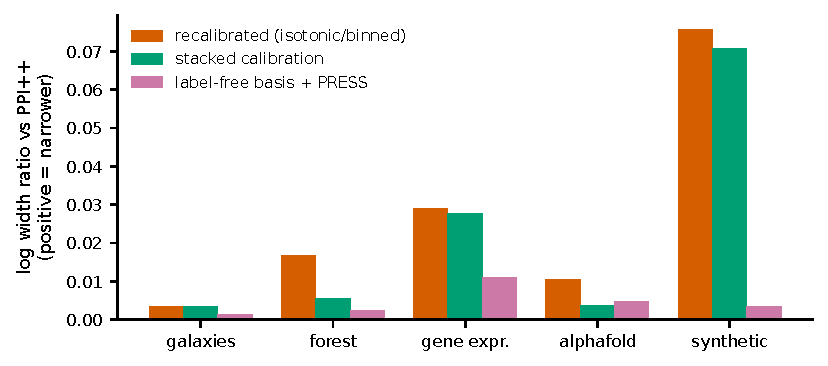
\includegraphics[width=\textwidth]{figures/search_variant_contrast.pdf}
\caption{Design-space contrast on the search pools: log width ratio against PPI++ for three model variants, five families, one evaluation per variant. Separate from, and not comparable in scale to, the sealed final results.}
\label{fig:search}
\end{figure}

\section{Discussion and Limitations}\label{sec:discussion}
\paragraph{What the evidence supports.} With fixed inputs, an interval narrower than PPI++ exists in the families we tested, but the average margin is about 2\% in width and the margin depends strongly on the pool: close to zero for the two other census pools (insurance, education) and a few percent for census income and the synthetic mixture. These margins come from the whole evaluated configuration (cross-fitted recalibration, Student-$t$ quantile, variance estimator and PPI++ fallback), none of whose components was ablated, so we do not attribute them to any single component. The population-level diagnostic is of the same sign and roughly the same size as the observed margin for the synthetic mixture and, less closely, for census income, but it predicts none for the plankton pool (a two-valued predictor whose unclipped optimal weight lies inside $[0,1]$), where the observed margin is 3.5\%, and it does not account for the observed gain in four of five families.

\paragraph{What it does not support.} The evidence does not show that the narrowing is free: coverage point estimates are 0.934 pooled and 0.91 for the lowest family, below 0.95, and the baselines' coverage is unknown. The observed gain exceeds the ceiling in four of five families, so part of it is not accounted for by the population-level diagnostic, and for plankton in particular the gain cannot be attributed to nonlinear calibration. The paper does not claim superiority beyond the pools evaluated, validity under the selection rule beyond the empirical gate, or generalization to other estimands or to covariate shift.

\paragraph{Limitations.} (1) Estimand: only the population mean at $\alpha=0.05$. (2) Sample sizes: $n=500$ on real pools and $n\in\{200,500\}$ on synthetic draws; no sweep over $n$ or $N$, although the theory predicts that small $n$ erodes the gain. (3) Single sealed run, no confidence intervals on width ratios, no per-episode widths or per-family coverage beyond the minimum in the artifacts, and no controlled ablation of the recalibrator, the second control variate, the Student-$t$ quantile or the selection rule. The mechanisms discussed above are therefore hypotheses. (4) The ceiling is a population-level asymptotic quantity computed with the evaluator's finite pools as the population; it is a diagnostic, not a bound on a finite draw. (5) The truth for real pools is the pool mean, with draws from the pool with replacement, so the evaluation checks inference for that finite population rather than for the original scientific population. (6) The evaluator's diagnostics for the candidate are marked as unverified. (7) The selection rule makes the interval data-dependent and the 1\% margin has no theoretical guarantee. (8) Stratified PPI is implemented but has no reported metrics and is not compared numerically.

\paragraph{Experiments that would test the hypotheses.} The mechanisms above can be tested with controlled comparisons that we did not run: (i) PPI++ with the weight clip removed, to separate the clipping component from nonlinear calibration; (ii) the recalibrated interval with the fallback disabled and with a fixed choice of recalibrator, to separate selection effects from the second control variate; (iii) the Student-$t$ quantile replaced by the normal quantile; (iv) coverage and width of every baseline, computed on the same draws and reported per family; and (v) a grid over $n$ and $N$ on the real pools, where the theory predicts a gain that shrinks with $n$ (estimation cost of order $p/n$) and with $r$. Until these are available, the decomposition in Section~\ref{sec:headroomcheck} should be read as a diagnostic of what is possible, not as an attribution of what the evaluated interval does.

\paragraph{Practical reading.} As a population-level computation, for census income about 84\% of the ceiling against PPI++ (0.0179 of 0.0213) is reachable by an unclipped linear weight on $\Yhat$, whereas in the synthetic nonlinear regime the ceiling arises from the nonlinearity of $\E[Y\mid\Yhat]$. This describes what is possible in the population, not what the evaluated interval does. Whether an unclipped PPI++ interval attains it, and at what coverage cost, was not tested here.

\section{Conclusion}
With labels, unlabeled data and predictor held fixed, the evaluated configuration (cross-fitted recalibration as a second control variate, Student-$t$ quantile and a PPI++ fallback) gave mean intervals 2.2\% narrower than PPI++ on average in a sealed evaluation, with reductions between 0.2\% and 4.0\% by family, and 6.8\% and 30\% narrower than PPI with $\lambda{=}1$ and the labeled-only interval. No component was ablated, so the gain is not attributed to recalibration. A closed-form population-level headroom diagnostic is small (aggregate 0.0129) and regime-dependent, and matches the observed margin closely only for the synthetic mixture and roughly for census income; it is zero for the plankton pool and does not account for the observed gain in four of five families. Coverage point estimates are 0.934 pooled and 0.91 for the lowest family, below the nominal 0.95, although the evaluator's tests did not reject. We read the result as conditional support for a small gain, not as evidence that PPI++ intervals can be shortened for free. The most useful next experiments are a coverage and width comparison of an unclipped PPI++ weight and each recalibration component in isolation, per-episode width and coverage reporting for all baselines, and a sweep over $n$.

% IMPORTANT: \clearpage flushes all pending floats before references so that
% body-page counting excludes reference-only pages.  Do NOT remove.
\clearpage
\bibliography{references}
\bibliographystyle{paper}

\clearpage
\appendix
\section{Supplementary Information}

\subsection{Source evidence and implementation details}\label{sec:si-source}
Implementation statements in this paper refer to the readable files in \texttt{source\_evidence/}: \texttt{frozen\_winner\_estimator.py} (the recalibrated interval), \texttt{variant\_label\_free\_basis\_estimator.py} and \texttt{variant\_stacked\_calibration\_estimator.py} (the two contrast variants), \texttt{evaluate\_final.py} and \texttt{evaluate\_search.py} (the two evaluators; the first has the SHA-256 recorded by the sealed evaluation), and \texttt{ppi\_py\_0.2.3\_excerpt.txt} (the reference PPI++ weight, which is clipped to $[0,1]$ when \texttt{clip=True}, the value used by the default mean interval). We assume the frozen file is the one evaluated in the sealed run, as recorded by the run manifest; hashes alone do not establish it.

Settings of the evaluated interval: $K=5$ shuffled folds seeded from the candidate's random generator; isotonic fit with clipped out-of-bounds prediction; binned fit with $\min(10,\max(2,\lfloor 0.8n/25\rfloor))$ bins (10 for $n=500$, 6 for $n=200$); pooled standardization of features; ridge $10^{-6}\,\mathrm{tr}(A)/p$ on the weight system; Student-$t$ quantile via a Cornish--Fisher expansion with degrees of freedom floored at 3; PPI++ weight clipped to $[0,1]$; fallback margin 0.99 applied to the PPI++ half-width only (the narrower of the isotonic and binned candidates is kept, with no margin between them). The evaluator enforces a 3\,s per-estimate deadline on the evaluated estimator.

\paragraph{Contrast variants.} The label-free basis variant uses a continuous piecewise-linear basis of $\Yhat$ with knots at pooled quantiles, the model size $p\in\{1,2,3,5,8\}$ is chosen by leave-one-out PRESS with a 2\% improvement margin, the standard error uses leverage-corrected leave-one-out residuals, and a guard keeps the width ratio against PPI++ above 0.85. The stacked variant fits seven calibrators (isotonic, three binned with 3, 5 and 8 bins, monotone and local-linear kernels, linear), combines them by non-negative least squares with 4 inner folds, repeats $K=5$ cross-fitting $R=5$ times under a time budget, and uses averaged-residual variance plus a split-dispersion term with $n-3$ degrees of freedom.

\subsection{Variance derivation}\label{sec:si-deriv}
For fixed $f,\lambda$, the two terms of $\hat\theta_\lambda$ are independent, so $V(\lambda)=\Var(Y-\lambda^\top f)/n+\Var(\lambda^\top f)/N$. Expanding, $nV(\lambda)=\Var(Y)-2\lambda^\top c+\lambda^\top\Sigma\lambda+r\lambda^\top\Sigma\lambda$, a quadratic with minimizer $\lambda^\star=\Sigma^{-1}c/(1+r)$ and minimum $\Var(Y)-c^\top\Sigma^{-1}c/(1+r)$. For $f=\Yhat$, $c^\top\Sigma^{-1}c=\Cov(Y,\Yhat)^2/\Var(\Yhat)=\rho^2\Var(Y)$. For $f=(\Yhat,m(\Yhat))$ the linear span contains $m$, and the squared multiple correlation of $Y$ on the span equals $\eta^2$. The PPI++ weight with its clip uses $\lambda=\mathrm{clip}(\Cov(Y,\Yhat)/((1+r)\Var(\Yhat)),0,1)$, whose variance is the quadratic evaluated at that point. These formulas are what the headroom script evaluates (\texttt{analysis/headroom.py}).

\subsection{Evaluator partitions}\label{sec:si-partition}
Figure~\ref{fig:partition} shows the five partition scores. Replicating the evaluator's episode plan shows that, after the first 30 draws, every family keeps the same reset seed, so each partition holds 76 draws of one family and 6 of every other. The scores mix large and very small per-family samples and should be read as a rough spread only.

\begin{figure}[t]
\centering
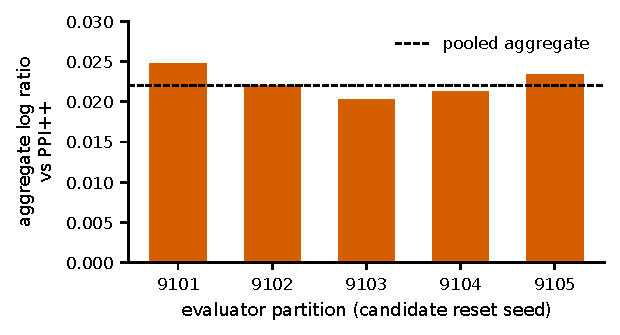
\includegraphics[width=0.62\textwidth]{figures/posthoc/headroom_partition_scores/partition_scores.pdf}
\caption{Aggregate log width ratio against PPI++ for each evaluator partition (candidate reset seed), with the pooled aggregate (dashed). Not independent replications.}
\label{fig:partition}
\end{figure}

\subsection{Search-pool metrics and sealed-evaluation details}
\begin{table}[h]
\centering
\caption{Search-pool metrics for the three model variants (single evaluation each): log width ratio against PPI++ by family, aggregate score, and coverage.}
\label{tab:search}
\small
\begin{tabular}{lrrrrrrrr}
\toprule
Variant & galax. & forest & gene & alpha. & synth. & agg. & cov.\ pooled & cov.\ min \\
\midrule
recalibrated & 0.0035 & 0.0168 & 0.0290 & 0.0104 & 0.0757 & 0.0271 & 0.943 & 0.933 \\
stacked & 0.0036 & 0.0054 & 0.0278 & 0.0038 & 0.0707 & 0.0223 & 0.943 & 0.917 \\
label-free basis & 0.0014 & 0.0024 & 0.0111 & 0.0049 & 0.0034 & 0.0046 & 0.950 & 0.933 \\
\bottomrule
\end{tabular}
% @evidence[[source_evidence/search_metrics/recalibrated_metrics.json]] @evidence[[source_evidence/search_metrics/stacked_metrics.json]] @evidence[[source_evidence/search_metrics/label_free_basis_metrics.json]]
\end{table}

Search pools: galaxy morphology (Galaxy Zoo-type crowd labels, \citealt{Willett2013GalaxyZ2}; $n=300$, $N=5000$), Amazon deforestation ($n=100$, $N=1000$), gene expression ($n=500$, $N=10000$), protein disorder ($n=300$, $N=5000$), and synthetic regimes, 60 draws per family, reset seeds 1001--1005. We cite an original data source only for the galaxy and census pools; the original sources of the plankton, deforestation, gene-expression and protein-disorder pools were not traced for this paper. The sealed evaluation plan declares 100 draws for each of five families (500 main episodes) plus 30 draws for each of two base pools and three control types (180 control episodes), 680 in total (constants \texttt{REPS\_MAIN} and \texttt{REPS\_CONTROL} in \texttt{source\_evidence/evaluate\_final.py}). The five recorded partitions have durations that sum to about 1332 seconds, against a wall-clock limit of 5400 seconds in the same script. % @evidence[[source_evidence/evaluate_final.py]] @evidence[[paper_data.json#final_evaluation.evaluation_evidence.episodes]]

\paragraph{Population quantities for the headroom check.} Table~\ref{tab:moments} lists the squared correlation and the correlation ratio per family.

\begin{table}[h]
\centering
\caption{Pool-level moments used for the ceiling (isotonic estimate of $\eta^2$; synthetic rows are large-sample regime moments). $\lambda^\star$ is the unclipped optimal weight on $\Yhat$ at $n=500$, $N=20000$, not applicable (---) to the synthetic regimes, which mix several $(n,N)$ cells.}
\label{tab:moments}
\small
\begin{tabular}{lrrrr}
\toprule
Pool or regime & $\rho^2$ & $\eta^2$ & $\eta^2-\rho^2$ & $\lambda^\star$ \\
\midrule
census income & 0.3691 & 0.3734 & 0.0044 & 1.342 \\
census insurance & 0.4996 & 0.5005 & 0.0009 & 0.961 \\
census education & 0.3921 & 0.3932 & 0.0011 & 0.953 \\
plankton (binary $\Yhat$) & 0.7004 & 0.7004 & 0.0000 & 0.841 \\
synthetic: linear calibrated & 0.5894 & 0.5895 & 0.0002 & --- \\
synthetic: nonlinear miscalibrated & 0.4831 & 0.7124 & 0.2292 & --- \\
synthetic: uninformative & 0.0000 & 0.0000 & 0.0000 & --- \\
synthetic: heteroscedastic & 0.7614 & 0.7616 & 0.0002 & --- \\
\bottomrule
\end{tabular}
% @evidence[[analysis/headroom_derived.json#real]] @evidence[[analysis/headroom_derived.json#synthetic_regimes]]
\end{table}

\subsection{Reproducibility}
The derived quantities are produced by \texttt{analysis/headroom.py} (reads the pool files, the evaluator's protocol constants and the sealed metrics, writes \texttt{analysis/headroom\_derived.json}) and the figures by \texttt{analysis/make\_figures.py}; both run in seconds on a CPU with NumPy, SciPy, scikit-learn and Matplotlib. Figure~\ref{fig:overview} is a schematic with no data. Table~\ref{tab:final} and Figure~\ref{fig:final} come from the sealed metrics plus the headroom file, Table~\ref{tab:search} and Figure~\ref{fig:search} from the search-pool metrics files, and Figure~\ref{fig:partition} from the sealed per-partition scores. The sealed evaluation itself is the external evaluator \texttt{evaluate\_final.py} run once on the frozen estimator, so it cannot be regenerated with different draws here. The synthetic ceilings use a fixed-seed Monte Carlo of $2\times10^6$ draws per regime.

\subsection{LLM Usage}
A large language model agent system was used throughout this study. It proposed the estimator designs, wrote and debugged the estimator code, ran the search-pool evaluations, wrote the headroom analysis and figure scripts, and drafted this manuscript. The task definition, the data pools and both evaluators were provided externally and were not modified; the sealed evaluation was run by the evaluator on the frozen estimator. All numbers in this paper come from the evaluator outputs or from the scripts cited above.

\end{document}
